% Masterthesis
%
% Multiscale Modelling Group of Jun.-Prof. Birgit Strodel
%
% Author:
% Oliver Schillinger


\ifdefined\isdraft
    \documentclass[english, a4paper, 12pt, titlepage, draft]{article}
\else
    \documentclass[english, a4paper, 12pt, titlepage, final]{article}
\fi

\usepackage{geometry}
\usepackage[british]{babel}
\usepackage{graphicx,hyperref,url,color,cite}
\usepackage{amsmath}
\usepackage[latin1]{inputenc}

\usepackage{setspace}
\usepackage[version=3]{mhchem}

\hypersetup{
    %bookmarks=false,                      % show bookmarks bar?
    unicode=true,                          % non-Latin characters in Acrobat’s bookmarks
    pdftoolbar=true,                       % show Acrobat’s toolbar?
    pdfmenubar=true,                       % show Acrobat’s menu?
    pdffitwindow=false,                    % window fit to page when opened
    pdfstartview={FitH},                   % fits the width of the page to the window
    pdftitle={Masterthesis},               % title
    pdfauthor={Oliver Schillinger},
    pdfsubject={Masterthesis},             % subject of the document
    pdfcreator={Oliver Schillinger},       % creator of the document
    pdfproducer={Oliver Schillinger},      % producer of the document
    pdfkeywords={Lipase} {CitA} {GROMACS}, % list of keywords
    pdfnewwindow=true,                     % links in new window
    colorlinks=true,                       % false: boxed links; true: colored links
    linkcolor=black,                       % color of internal links
    citecolor=blue,                        % color of links to bibliography
    filecolor=red,                         % color of file links
    urlcolor=cyan                          % color of external links
}


% Figure template
%\begin{figure}
%    \centering
%    
\includegraphics[width=0.5\textwidth]{figures/draft/draft.pdf}
%    \caption{}
%    \label{fig:}
%\end{figure} 


% ============================================================================ %


\begin{document}

% ============================================================================ %

\begin{titlepage}
\begin{center}
{\huge \textbf{Masterthesis}}\\
\vspace{2cm}
{\large \textbf{Protein Structure and Dynamics} \\
\vspace{1cm}
of \textit{Bacillus Subtilis} Lipase LipA Fused to the Ligand-Binding Domain of Sensor Histidine Kinase CitA
}

\vspace{2cm}

Oliver Schillinger \\
Forschungszentrum J\"ulich \\ Institute of Complex Systems 6 - Structural Biochemistry \\ Multiscale Modelling Group \\
Supervisor: Jun.-Prof. Dr. Birgit Strodel \\
\vspace{1cm}
German Research School for Simulation Sciences \\
RWTH Aachen

\vspace{1cm}

\today

\vfill

\begin{figure}[h!]

\includegraphics[width=.3\textwidth]{figures/logos/grs_logo.pdf}
\hspace{0.5cm}

\includegraphics[width=.3\textwidth]{figures/logos/fzj_logo.pdf}
\hspace{0.5cm}

\includegraphics[width=.3\textwidth]{figures/logos/rwth_logo.pdf}
\end{figure}
 
\end{center}
\end{titlepage}


% ============================================================================ %

\onehalfspacing

\begin{abstract}

The structure and kinetics of two proteins under investigation are well known:
The periplasmic domain of sensor \textit{Klebsiella pneumoniae} histidine kinase CitA (PDB accession code \href{http://pdb.rcsb.org/pdb/explore/explore.do?structureId=2J80}{2J80}) \cite{CitA_2J80}
and the lipase LipA of \textit{Bacillus subtilis} (BSLA, PDB accession code \href{http://pdb.rcsb.org/pdb/explore/explore.do?structureId=1I6W}{1I6W}), \cite{BSLA_1I6W} both in their ligand bound and ligand free states.
What is not understood is the structure and kinetics of a fusion protein of these two peptides.
Experiments indicate that citrate binding to the kinase down-regulates lipase activity (Figure \ref{fig:BSLAactivity}).
This effect is of major interest to the chemical industry as lipases exhibit a wide diversity in substrate specificity and have found applications in the resolution of racemic mixtures, the synthesis of esters, transesterification reactions and as additives in laundry detergents.
As chemical applications would benefit from the opposite effect, a controlled up-regulation of lipase activity triggered by citrate addition, this research focused on the structure elucidation of the fused protein, as well as on the mechanism by which lipase activity is regulated.
A thorough understanding of this mechanism might in the future enable us to engineer the protein to invert the regulatory effect of citrate binding.
The main methods used for structure elucidation are global optimization using the Monte Carlo-minimization approach basin hopping, followed by high-throughput molecular dynamics simulations. 

\end{abstract}


% ============================================================================ %

\tableofcontents

\pagebreak

\onehalfspacing

% ============================================================================ %

\section{Introduction}

\begin{figure}
    \centering
    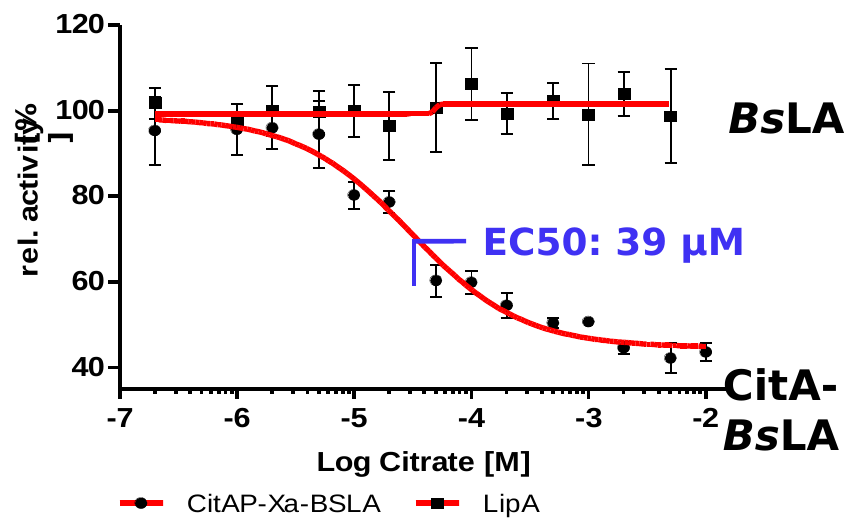
\includegraphics[width=0.5\textwidth]{figures/BSLA_activity/BSLA_activity.png}
    \caption{The activity of the BSLA -- CitA complex is reduced after citrate addition while the uncomplexed lipase is not affected. Experiments performed by Karl Erich Jaeger et al., data unpublished.}
    \label{fig:BSLAactivity}
\end{figure}


% ============================================================================ %

\section{Proteins Under Investigation}

% ==================================== %

\subsection{\textit{Bacillus Subtilis} Lipase LipA}

\textit{Bacillus Subtilis} is a gram-positive, aerobic bacterium found in soil and water, that is subject to active research since 1992 \cite{bacillusSubtilis}.
\textit{Bacillus Subtilis} is of major industrial interest because of its highly efficient protein secretion system \cite{BSsecretion} enabling the production of proteases and amylases in bulk quantities \cite{BSworkhorse}.
Of special interest are its excreted lipases, as these catalyze the hydrolysis and synthesis of long chain triacylglycerols \cite{BSLA_1I6W}.
These lipases possess a wide substrate specificity.
They find applications in transesterification reactions, the synthesis of esthers, the resolution of racemic mixtures and are used as additives in laundry detergents \cite{BSdetergents}.

The reported experiments where performed using lipase LipA from \textit{Bacillus Subtilis} (BSLA).
Compared to lipases from other organisms BSLA is relatively small, consisting of 181 amino acids and weighting slightly more than 19 kDA.
BSLA belongs to the $\alpha$-$\beta$ hydrolase fold enzymes.
Members of this protein family are constituted by a twisted $\beta$-strand core flanked by alpha helices on both sides \cite{alphaBetaHydrolases}.
Because of its small size and because other known $\alpha$-$\beta$ hydrolase fold enzymes extend on this core structure, it can be considered a minimal $\alpha$-$\beta$ hydrolase.
BSLA hydrolyses sn-1 and sn-3 glycerol esthers with long fatty acid chains, while its highest activity is exhibited on medium sized fatty acids \cite{BSLA_1I6W}.
The optimum environment is reported to be found at pH 10 \cite{BSLA_1I6W}.

Most known lipases possess an $\alpha$-helical segment that covers the active site.
The encounter of lipid-aggregates triggers the opening of this lid, exposing the active site and triggering catalytic activity.
This behaviour is known as interfacial activation \cite{alphaBetaHydrolases}.
BSLA lacks this lid, resulting in an active site that is solvent exposed and thus activlely hydrolising fatty acids even in the absence of lipid-aggregates.

The active site is located at the bottom of a shallow cleft formed by four turns (Figure \ref{fig:BSLAactiveSite}).
Its structure is in accordance with the secondary structure topology of the canonical $\alpha$/$\beta$-hydrolase fold, in which the acitve site is formed by a nucleophile, an acid and a histidine, together called the catalytic triad \cite{BSLA_1I6W}.
In BSLA this catalytic triad is constituted of Ser77 (nucleophile), Asp133 (acid) and His156.
Serine 77 is located at the so called nucleophilic elbow \cite{nucleophileElbow}, a sharp turn at the bottom of the binding pocket connecting a central $beta$-sheet to a peripheral $\alpha$-helix.
The ester hydrolysis catalyzed by BSLA is depicted in Figure \ref{fig:BSLAreaction}.
The ligand binds covalently with its phosphoryl group to Ser77.
A tetrahedral intermediate structure is formed.
One phosphoryl oxygen of the substrate is hydrogen bound to the \ce{NH} atoms of Met78 and Ile12, forming the oxyanion hole that is common to most lipases \cite{BSLA_1I6W}.
The \ce{N^{$\epsilon$}} atom of His156 is located at hydrogen bonding distance from the Ser77 \ce{O^{$\gamma$}} atom and the substrate esther oxygen.






\begin{figure}
    \centering
    
\includegraphics[width=0.5\textwidth]{figures/draft/draft.pdf}
    \caption{Active site of \textit{Bacillus Subtilis} lipase LipA.}
    \label{fig:BSLAactiveSite}
\end{figure} 

\begin{figure}
    \centering
    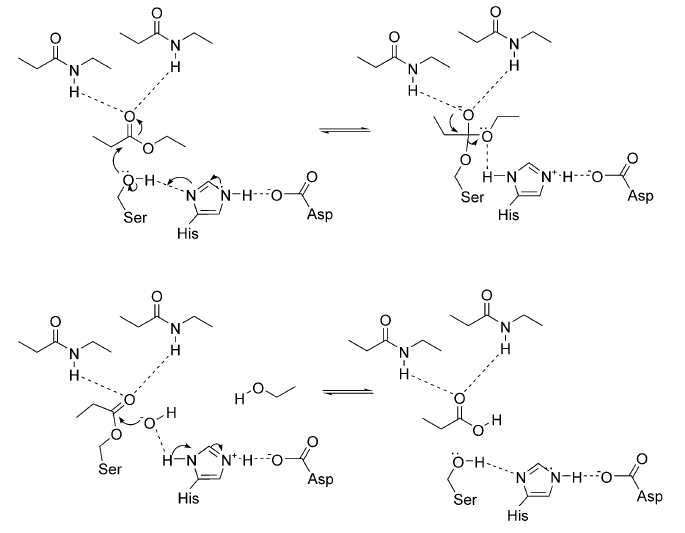
\includegraphics[width=0.7\textwidth]{figures/BSLA_reaction.png}
    \caption{Ester hydrolysis reaction catalyzed by BSLA. Taken from \cite{BSLA_reaction}.}
    \label{fig:BSLAreaction}
\end{figure}  





% ==================================== %

\subsection{Periplasmic Domain of Sensor Histidine Kinase CitA}

CitA is the sensor histidine kinase of a two component regulatory system of \textit{Klebsiella Pneumoniae} \cite{CitA_original}.
These systems generaly consist of a sensor histidine kinase and a response regulator (CitB in the present case).
Sensor histidine kinases respond to environmental conditions by autophosphorilation of a conserved histidine residue.
The phosphoryl group is subsequently transferred to a conserved Aspartate residue on the response regulator.
The phosphorylated response regulator in turn triggers a change in gene expression or cell behaviour \cite{CitA_original}.
The CitA/CitB regulatory system controls the expression of citrate frementation genes.
Citrate metabolims requires careful regulation, as an uncontrolled upregulation in the absence of citrate would break the citric acid cycle with servere consequences for the organism \cite{CitA_original}.

Like most known sensor histidine kinases, CitA is a membrane protein, the domain composition of which is shown in Figure \ref{fig:CitA_organization}.
Its extracellular N-terminal sensor domain is flanked by two transmembrane helices, one of which links to the intracellular autokinase domain.
Like virtually all known sensor histidine kinases, CitA appears to be dimeric \cite{2CST}.
In many cases only the structures of extracellular domains of sensor kinases are known, due to the inherent difficulties of obtaining structural information about membrane proteins.
This is also true for CitA, where only structures of the periplasmic domain (CitAP) have been resolved.
The overall fold of the periplasmic domain of sensor histidine kinases classifies them as members of the Per-Arnt-Sim domain superfamily.
This superfamily comprises many well studied sensor histidine kinases \cite{PAS}.


\begin{figure}
    \centering
    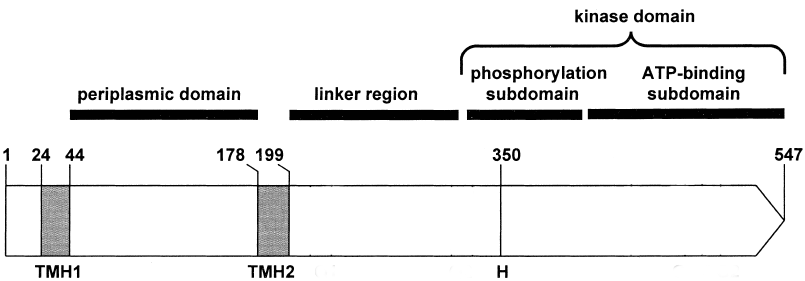
\includegraphics[width=0.7\textwidth]{figures/CitA_organization.png}
    \caption{CitA domain organization. Only the structure of the periplasmic domain (CitAP) is known and was used in the reported research. Histidine 350 gets phosphorylated after signal transduction as described in the text. Figure taken from \cite{CitA_original}}
    \label{fig:CitA_organization}
\end{figure}   


The mechanism of action of CitA \cite{CitA_original} is initiated by citrate binding, triggering a conformational change of the periplasmic domain that is mediated by a transmembrane helix to the cytoplasmic kinase domain.
It has been hypothesized that this mediation happens by a piston-like mechanism (see Figure \ref{fig:CitA_mechanism}) in which transmembrane helix 2 is pulled out of the membrane.
The resulting conformational change in the kinase domain allows the interaction of the ATP-binding subdomain with the cytoplasmic phosphorylation subdomain.
After autophosphorylation the subdomains dissociate.
The phosphorylation subdomain can now bind to the receiver domain of the response regulator CitB.
A final phosphotransfer on the phosphorylation domain from histidine to an aspartate completes the CitA cycle and new response can be triggered.


\begin{figure}
    \centering
    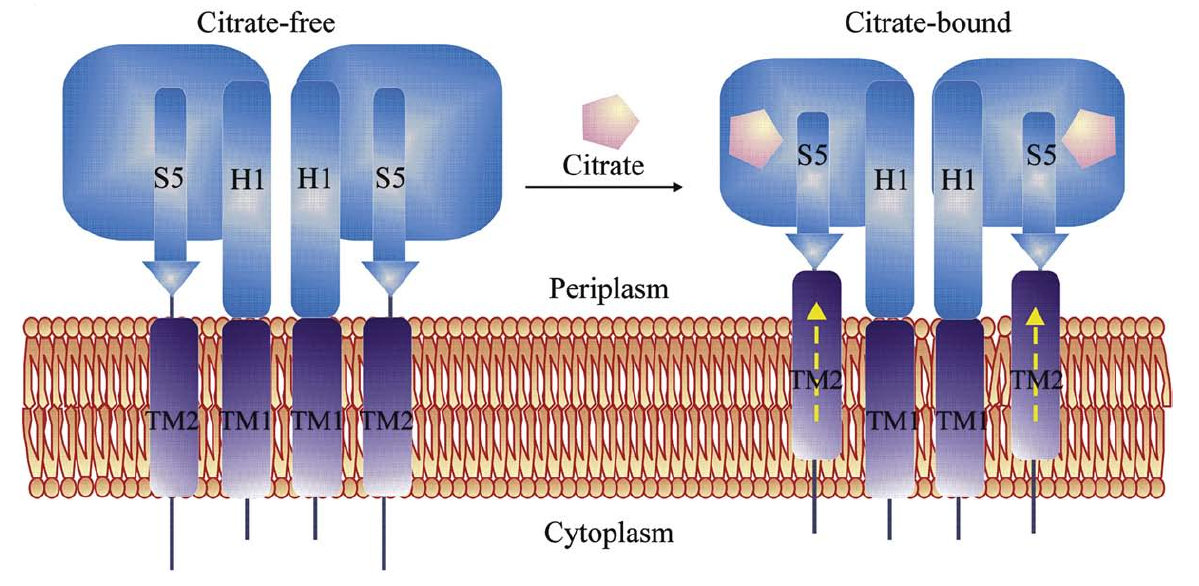
\includegraphics[width=0.7\textwidth]{figures/CitA_mechanism.png}
    \caption{Hypothetical mode of action of CitA. The citrate triggered conformational change of the periplasmic domain is mediated to the cytoplasmic kinase domain by a piston-like mechanism. Figure taken from \cite{CitA_2J80}}
    \label{fig:CitA_mechanism}
\end{figure}    



The binding pocket of CitAP build up from the $\beta$-sheet core that forms the bottom and two loops, the minor loop (residue 96 to 106) and the major loop (residue 63 to 92).
These loops form tight lids covering the bound ligand and forming a closed pocket.
While the \textit{in vivo} conformation of the termini remains uncertain due to crystal packing artifacts the core structure of the bound CitAP has been solved with 1.6 $\mathring{A}$ resolution and has been experimentally found to be well folded in solution \cite{CitA_2J80}.
The major loop is unresolved in the unbound CitAP structures, indicating that it is highly mobile without the stabilizing effect of the ligand.
The core structure of the protein is highly similar for the bound and unbound structures with similar backbone positions and sidechain orientations of the binding residues not located in the loops \cite{CitA_2J80}.
A sodium ion has been crystalized in the citrate bound structures.
Its physiological significance had already been indicated by the fact that sodium is required for the induction of the CitA/CitB target genes \cite{KlebsiellaMetabolism} and is backed by the by the fact that no sodium has been found in the citrate free crystal structure.

It has been reported that citrate binding to CitA is highly specific and that virtually all CitA is in the bound state under physiological citrate concentrations \cite{CitA_2J80}.
Citrate interacts mainly with Thr58, Arg66, His69, Glu80, Ser101, Leu102, Arg107, Lys109 and Ser124 by hydrogen bonding (\ref{fig:citrate_interactions}).
A further hydrogen bond is mediated by a water molecule to Gly103.
The conformational change in the periplasmic domain of sensor histidine kinase CitA is illustrated in Figure \ref{fig:CitA_opening}.
The main conformational change is the flattening of the $\beta$-sheet that forms the minor loop.
Upon citrate binding this $\beta$-sheet is pulled in due to interaction with the ligand.
This disrupts some of the interactions with neighbouring $\beta$-sheets and subsequently pulls the C-terminus away from the membrane.
The unstructured major loop in the citrate free crystal structure indicates that the citrate binding pocket is less stable when citrate is not present.


\begin{figure}
    \centering
    
\includegraphics[width=0.5\textwidth]{figures/draft/draft.pdf}
    \caption{The conformational change in the periplasmic domain of sensor histidine kinase CitA.
    The closed conformation has been taken from the citrate bound structure with PDB accession code \href{http://pdb.rcsb.org/pdb/explore/explore.do?structureId=2J80}{2J80}.
The open conformation is a snapshot from a 100 ns molecular dynamics simulation in which the citrate had been removed.}
    \label{fig:CitA_opening}
\end{figure}     



\begin{figure}
    \centering
    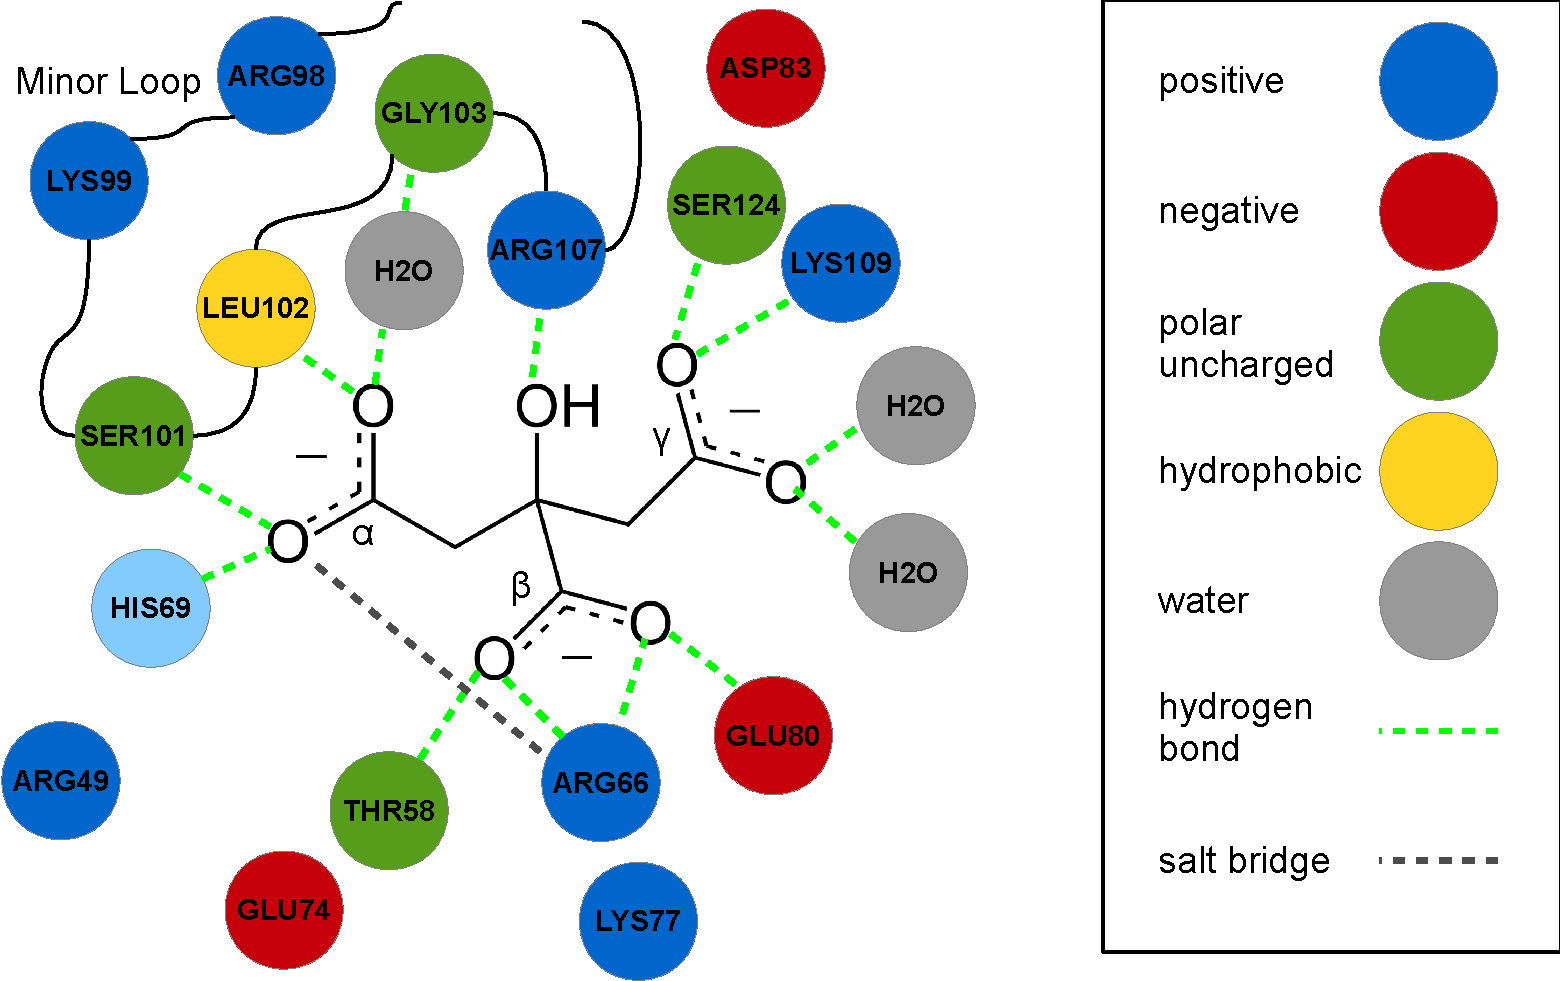
\includegraphics[width=0.7\textwidth]{figures/citrate_interactions/citrate_interactions.pdf}
    \caption{Interactions of CitA with its bound ligand citrate as determined by visual inspection of a 1ns molecular dynamics trajectory. The minor loop is the domain with the largest RMSD during active site opening.}
    \label{fig:citrate_interactions}
\end{figure}      


% ==================================== %

\subsection{Fusion Complex}


% ============================================================================ %

\section{Methods}
\subsection{Molecular Dynamics}

The main method that was be used in the presented research is Molecular Dynamics simulations (MD) based on classical Molecular Mechanics (MM) \cite{MDintro}.
In Molecular Mechanics molecules are modelled as systems of chemically inert atoms that interact through Newtonian mechanics.
The interaction energy between atoms is described by preferably simple mathematical equations, mainly harmonic and trigonometric functions, as well as the well known electrostatic and Lennard-Jones potentials.
A given set of potential energy formulas, together with its parameters, is called a force field, as it is used to compute the interatomic forces.
These forces are then numerically integrated to obtain a trajectory in phase-space.
This trajectory can in turn be used to estimate thermodynamic quantities (e.g. free energies), as well as to derive dynamic properties, such as normal modes of protein movement \cite{normalModes}.
Molecuar Dynamics has been successfully used to study biomolecules for more than 35 years \cite{MDbiomolecules}.

A great variety of force fields exists and a careful and well informed choice about the set of equations and parameters that can model the system under investigation best has to be made.
Recent benchmarks of protein force fields give insights into the strengths and weaknesses of the available options \cite{proteinFF}, indicating that one of the most up to date corrections to the widely used amber force field \cite{amber99sb-ildn-nmr} is the best choice for simulations of proteins.

To analyze the obtained data a large variety of methods exist ranging from hydrogen bond network and interaction energy analysis to principal component and normal mode analysis, to name just a few.
 
\subsubsection{Force Fields}
\subsubsection{Water Model}
\subsection{Basin Hopping with GMIN}
%\subsection{pKa Prediction}
\subsection{k-Means Clustering}


% ============================================================================ %

\section{Simulation Setups}

All citrate bound CitA structures in the PDB contain a specific sodium ion attached to the first $\alpha$-helix as well as 3 water molecules in similar orientations in the vicinity of citrate.
This regularity makes it probable that these molecules might fulfill an active roll in CitA's dynamics.
They have therefore been included in the simulation setups.

\subsection{Equilibration}
\subsection{Production Runs}


% ============================================================================ %

\section{Results}


% ============================================================================ %

\section{Discussion \& Conclusion}


% ============================================================================ %

\section{Outlook}
The results should be combined with experimental data from small angle X-ray scattering, and NMR experiments. The mechanism of activity regulation is investigated with the help of non-equilibrium molecular dynamics.


% ============================================================================ %

\section{Acknowledgments}

% ============================================================================ %

\section{Declaration of Authorship}

% \declareAuthorship{date}{place}{name}
% date is optional and defaults to \today
\newcommand{\declareAuthorship}[3][\today]{

    \noindent
    I, #3, hereby declare that I have created this work completely on my own and
    used no other sources or tools than the ones listed, and that I have marked
    any citations accordingly.  

    \begin{minipage}[c]{\textwidth}

        \vspace{2cm}

        \makebox[\textwidth][c]{
            \makebox[.4\textwidth][l] {\textrm{#2, #1}}
            \hfill
            \makebox[.4\textwidth][c] {\hrulefill}
            \hfill
        }
        \makebox[\textwidth][c]{
            \hfill
            \makebox[.4\textwidth][c] {}
            \emph{#3}
            \hfill
        }
        \vspace{1cm}
    \end{minipage}
}

\declareAuthorship{J\"ulich}{Oliver Schillinger}



% ============================================================================ %

\singlespacing
\small

\bibliographystyle{unsrt}
\bibliography{masterthesis}
 
% ============================================================================ %

\end{document}
 
